

%-------------------------------------------------------------------------------
% Dokumenten Klasse
\documentclass[
	final,
	a4paper,
	oneside,
	parskip=full,
	headings=standardclasses,
	headings=big,
	pointednumbers
]{scrartcl}

%-------------------------------------------------------------------------------
% Packete nutzen
\usepackage{ngerman,palatino,setspace}
\usepackage[T1]{fontenc}
\usepackage[utf8]{inputenc}
\usepackage[left=20mm,right=20mm,top=25mm,bottom=25mm]{geometry}
\usepackage{amsmath}
\usepackage{mathtools}
\usepackage{tikz}

\usetikzlibrary{automata, positioning, arrows}

%{
%\tikzset{
%    ->, % makes the edges directed
%    >=stealth, % makes the arrow heads bold
%    node distance=2cm, % specifies the minimum distance between two nodes. Change if necessary.
%    every state/.style={thick, fill=gray!10}, % sets the properties for each ’state’ node
%    every edge/.append style={line width=0.25mm}, % sets the properties for each ’state’ node
%    initial text=$ $, % sets the text that appears on the start arrow
%}
%}

\tikzset{
    node distance=2cm, % Minimum distance between two nodes. Change if necessary.
    every state/.style={ % Sets the properties for each state
        semithick,
        fill=gray!10
    },
    initial text={}, % No label on start arrow
    double distance=2pt, % Adjust appearance of accept states
    every edge/.style={ % Sets the properties for each transition
        draw,
        ->,>=stealth, % Makes edges directed with bold arrowheads
        auto,
        semithick
    },
    shift left/.style ={commutative diagrams/shift left={#1}},
    shift right/.style={commutative diagrams/shift right={#1}}
}

%-------------------------------------------------------------------------------
\usepackage{multirow}

%-------------------------------------------------------------------------------
% uline
\usepackage{ulem}

%-------------------------------------------------------------------------------
% Anderer Font
\usepackage{mathrsfs}
\usepackage[mathcal]{euscript}

%-------------------------------------------------------------------------------
% Square brackets
\usepackage{stmaryrd}

%-------------------------------------------------------------------------------
% Dokument
\begin{document}
    
    
    %--- Page 1 --------------------------------------------------------------------
    
   	
    \begin{minipage}{0.1\textwidth}
       ab:
   	\end{minipage}
   	\begin{minipage}{0.9\textwidth}
       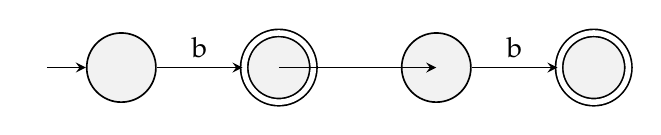
\begin{tikzpicture}
           \node[state, initial left]                  (aq1)    {};
           \node[state, accepting, right of=aq1]       (aq2)    {};
           \node[state, right of=aq2]                  (bq1)    {};
           \node[state, accepting, right of=bq1]       (bq2)    {};
           \coordinate (x) at (aq2);
           \coordinate (y) at (bq1);
           \draw   (aq1) edge[]        node{b} (aq2)
                   (bq1) edge[]        node{b} (bq2)
                   (x) edge (y)
           ;
       \end{tikzpicture}
   	\end{minipage}
       
   	\begin{minipage}{0.1\textwidth}
        ab:
   	\end{minipage}
   	\begin{minipage}{0.9\textwidth}
        \begin{tikzpicture}
            \node[state, initial left]                  (aq1)    {};
            \node[state, accepting, right of=aq1]       (aq2)    {
            \begin{tikzpicture}
                \draw (0,0) -- (0,1);
            \end{tikzpicture}};
            \node[state, right of=aq2]                  (bq1)    {};
            \node[state, accepting, right of=bq1]       (bq2)    {};
            \draw   (aq1) edge[]        node{b} (aq2)
                    (bq1) edge[]        node{b} (bq2)
            ;
        \end{tikzpicture}
   	\end{minipage}
    

\end{document}
